\documentclass[crop,tikz]{standalone}
\usepackage{amsmath}

\usetikzlibrary{
	chains,
	positioning,
	arrows.meta,
	decorations.pathreplacing,
	calc,
	fit,
	shapes.geometric
}

\begin{document}

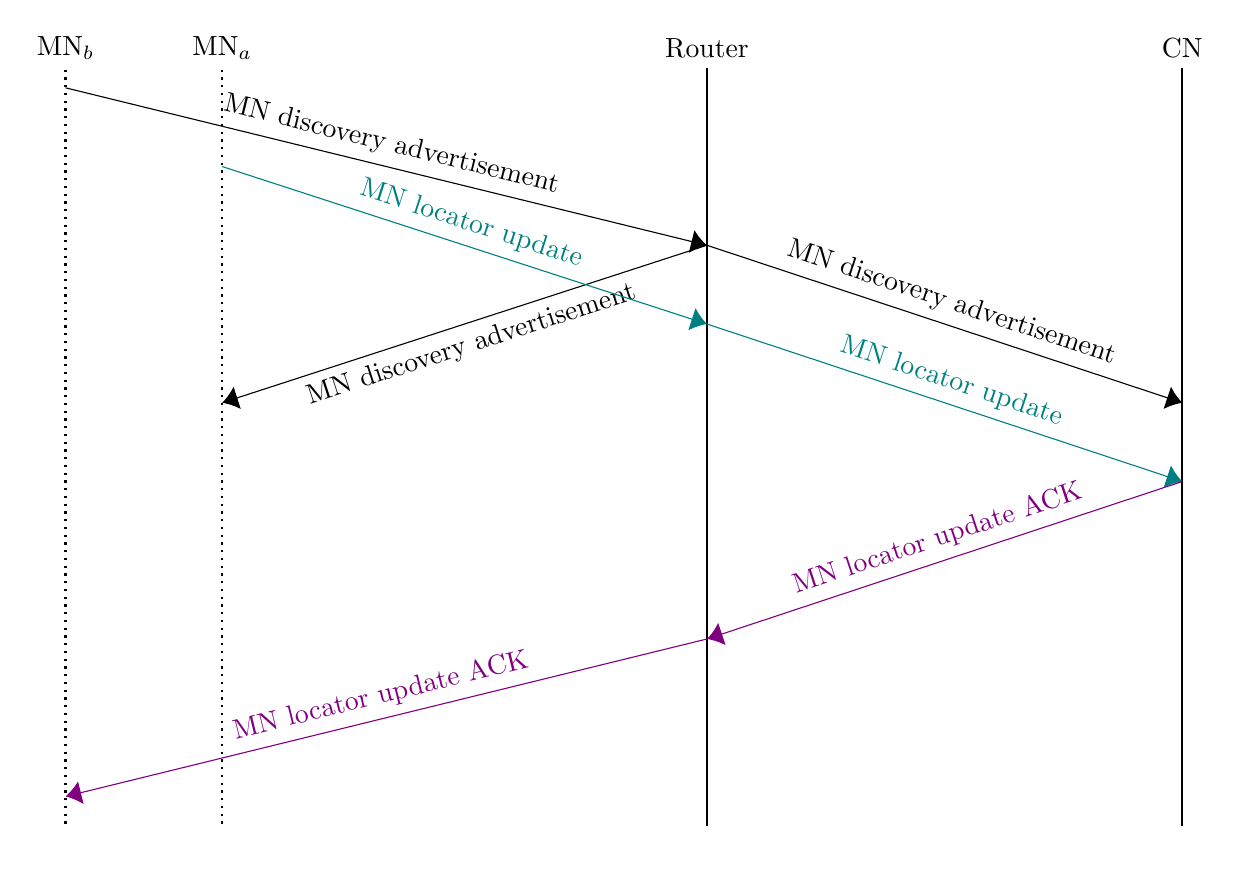
\begin{tikzpicture}[]
	\node[] (r) {Router};
	\node[right = 5cm of r] (cn) {CN};
	\node[left = 5cm of r] (mna) {$\text{MN}_a$};
	\node[left = 1cm of mna] (mnb) {$\text{MN}_b$};
	\node[below of=r, node distance=10cm] (r_ground) {};
	\node[below of=cn, node distance=10cm] (cn_ground) {};
	\node[below of=mnb, node distance=10cm] (mnb_ground) {};
	\node[below of=mna, node distance=10cm] (mna_ground) {};

	\draw[thick] (r) -- (r_ground);
	\draw[thick] (cn) -- (cn_ground);
	\draw[dotted, thick] (mnb) -- (mnb_ground);
	\draw[dotted, thick] (mna) -- (mna_ground);
		
	\draw[-{Latex[length=2mm,width=3mm]}] ($(mnb)!0.05!(mnb_ground)$) -- node[above,sloped]{MN discovery advertisement}  ($(r)!0.25!(r_ground)$);
	\draw[-{Latex[length=2mm,width=3mm]}] ($(r)!0.25!(r_ground)$) -- node[below,sloped]{MN discovery advertisement}  ($(mna)!0.45!(mna_ground)$);
	\draw[-{Latex[length=2mm,width=3mm]}] ($(r)!0.25!(r_ground)$) -- node[above,sloped]{MN discovery advertisement}  ($(cn)!0.45!(cn_ground)$);
	
	\draw[-{Latex[length=2mm,width=3mm]},teal] ($(mna)!0.15!(mna_ground)$) -- node[above,sloped]{MN locator update}  ($(r)!0.35!(r_ground)$);
	\draw[-{Latex[length=2mm,width=3mm]},teal] ($(r)!0.35!(r_ground)$) -- node[above,sloped]{MN locator update}  ($(cn)!0.55!(cn_ground)$);
	
	\draw[-{Latex[length=2mm,width=3mm]},violet] ($(cn)!0.55!(cn_ground)$) -- node[above,sloped]{MN locator update ACK}  ($(r)!0.75!(r_ground)$);
	\draw[-{Latex[length=2mm,width=3mm]},violet] ($(r)!0.75!(r_ground)$) -- node[above,sloped]{MN locator update ACK}  ($(mnb)!0.95!(mnb_ground)$);
\end{tikzpicture}

\end{document}